\documentclass[conference]{IEEEtran}

\usepackage{cite}
\usepackage{amsmath,amssymb,amsfonts}
\usepackage{graphicx}
\usepackage{textcomp}
\usepackage{xcolor}
\usepackage{float}
\usepackage{booktabs}
\usepackage{multirow}
\usepackage{enumerate}
\usepackage{hyperref}
\hypersetup{colorlinks=true,linkcolor=black,citecolor=black,urlcolor=blue}

\newcommand{\um}{\,$\mu$m}
\newcommand{\umsq}{\,$\mu$m$^2$}
\newcommand{\cell}[1]{\texttt{\detokenize{#1}}}

\begin{document}

\title{4-Bit Array Multiplier from RTL to GDSII\\ with Open-Source Tools\\
\large Digital VLSI Design (M26EC2.408) Assignment Report (Team Madhurbala\_riders)}

\author{\IEEEauthorblockN{Vansh Jaiswal}
\IEEEauthorblockA{
\textit{ECE, IIIT Hyderabad}\\
2024102013\\
vansh.jaiswal@students.iiit.ac.in}
\and
\IEEEauthorblockN{Saarthak Sabharwal}
\IEEEauthorblockA{
\textit{ECE, IIIT Hyderabad}\\
2023102055\\
saarthak.sabharwal@students.iiit.ac.in}
}

\maketitle

\begin{abstract}
This report presents the design, verification and complete open-source RTL-to-GDSII implementation of a
registered 4-bit $\times$ 4-bit unsigned array multiplier in the SkyWater SKY130 130\,nm process with the
\cell{sky130_fd_sc_hd} standard-cell library. The multiplier, built from 16 AND gates and 12 full adders between
an input and an output register, is verified exhaustively in RTL and gate-level simulation (256/256 vectors).
Yosys maps it to 63 cells (740.71\umsq, flip-flops 54.05\,\% of the area); OpenSTA gives a minimum period of
2.604\,ns (384.0\,MHz) at the typical corner, with a critical path through 7 full-adder stages. LibreLane
then places and routes the design on a 150\,$\times$\,150\um\ die with 0 DRC and 0 LVS errors, closing
multi-corner setup timing at a 6.5\,ns clock (post-route $F_{max}$ 155.9\,MHz). The gap between the
pre-layout and post-route frequency is analysed in terms of process corners, interconnect, the clock tree
and the cells added by the physical-design flow.
\end{abstract}

\section{Introduction}
Multiplication is a core operation in arithmetic and signal-processing datapaths. The array multiplier is
the most regular hardware realisation of shift-and-add multiplication: every partial product is formed by
a row of AND gates and the rows are summed by ripple-carry adders laid out as a two-dimensional array. Its
regularity makes it a good vehicle for exercising a complete design flow, while its carry chains give a
clearly identifiable critical path whose length grows linearly with the word length.

In this assignment a registered 4-bit array multiplier is taken through the full open-source flow:
\begin{itemize}
    \item RTL design and exhaustive self-checking simulation (Icarus Verilog, GTKWave),
    \item logic synthesis to SKY130 standard cells (Yosys) and gate-level simulation,
    \item static timing analysis (OpenSTA),
    \item floorplanning, placement, clock-tree synthesis, routing and signoff (LibreLane with OpenROAD,
          Magic, KLayout and Netgen), producing the final GDSII layout.
\end{itemize}
All tools were run from the IIC-OSIC-TOOLS Docker image~\cite{iic}. The exact command for every step is
listed in the repository \texttt{README.md}.

\section{Theory and Proposed Design}

\subsection{Partial Products}
For two 4-bit unsigned operands $A=a_3a_2a_1a_0$ and $B=b_3b_2b_1b_0$, multiplication is
shift-and-add~\cite{weste,rabaey}.
Each bit $b_i$ of the multiplier selects one partial product
\begin{equation}
pp_i[j] = a_j \wedge b_i, \qquad i,j \in \{0,\dots,3\},
\end{equation}
which is weighted by $2^i$, so that
\begin{equation}
P = \sum_{i=0}^{3} 2^{i} \sum_{j=0}^{3} 2^{j}\, pp_i[j], \qquad 0 \le P \le 225 .
\end{equation}

\subsection{Array Structure}
The array adds the partial products one row at a time:
\begin{enumerate}
    \item Row 0 consists only of AND gates. Its lowest bit is the final product bit $p_0 = pp_0[0]$ and the
          other three bits are passed down as $r_0 = \{0,\,pp_0[3],\,pp_0[2],\,pp_0[1]\}$.
    \item Rows $i = 1,2,3$ are 4-bit ripple-carry adders. Full adder $j$ of row $i$ adds $pp_i[j]$, $r_{i-1}[j]$
          and the carry $c_i[j]$ (with $c_i[0]=0$), producing the sum $s_i[j]$ and the carry $c_i[j+1]$.
    \item The lowest sum bit of each row is a finished product bit, $p_i = s_i[0]$, and the row passes down
          $r_i = \{c_i[4],\,s_i[3],\,s_i[2],\,s_i[1]\}$.
    \item The last row also gives the top four product bits, $p_{7:4} = r_3$.
\end{enumerate}
Each full adder computes
\begin{align}
s &= a \oplus b \oplus c_{in}, \\
c_{out} &= ab + a\,c_{in} + b\,c_{in}.
\end{align}
In general an $N$-bit array multiplier needs $N^2$ AND gates and $N(N-1)$ full adders, i.e.\ 16 AND gates
and 12 full adders for $N=4$, and its longest path is roughly $2N$ full-adder delays.

\subsection{Registers and Latency}
The operands are registered into \texttt{a\_r} and \texttt{b\_r} on every rising clock edge, the array is
built from the registered values, and the 8-bit result is registered into \texttt{p}. This gives exactly
16 flip-flops, all with an asynchronous active-low reset \texttt{rst\_n}. An input applied before clock
edge~1 is captured at edge~1 and the product appears at edge~2: the latency is 2 clock cycles and the
throughput is one product per cycle.

\begin{figure*}[t]
    \centering
    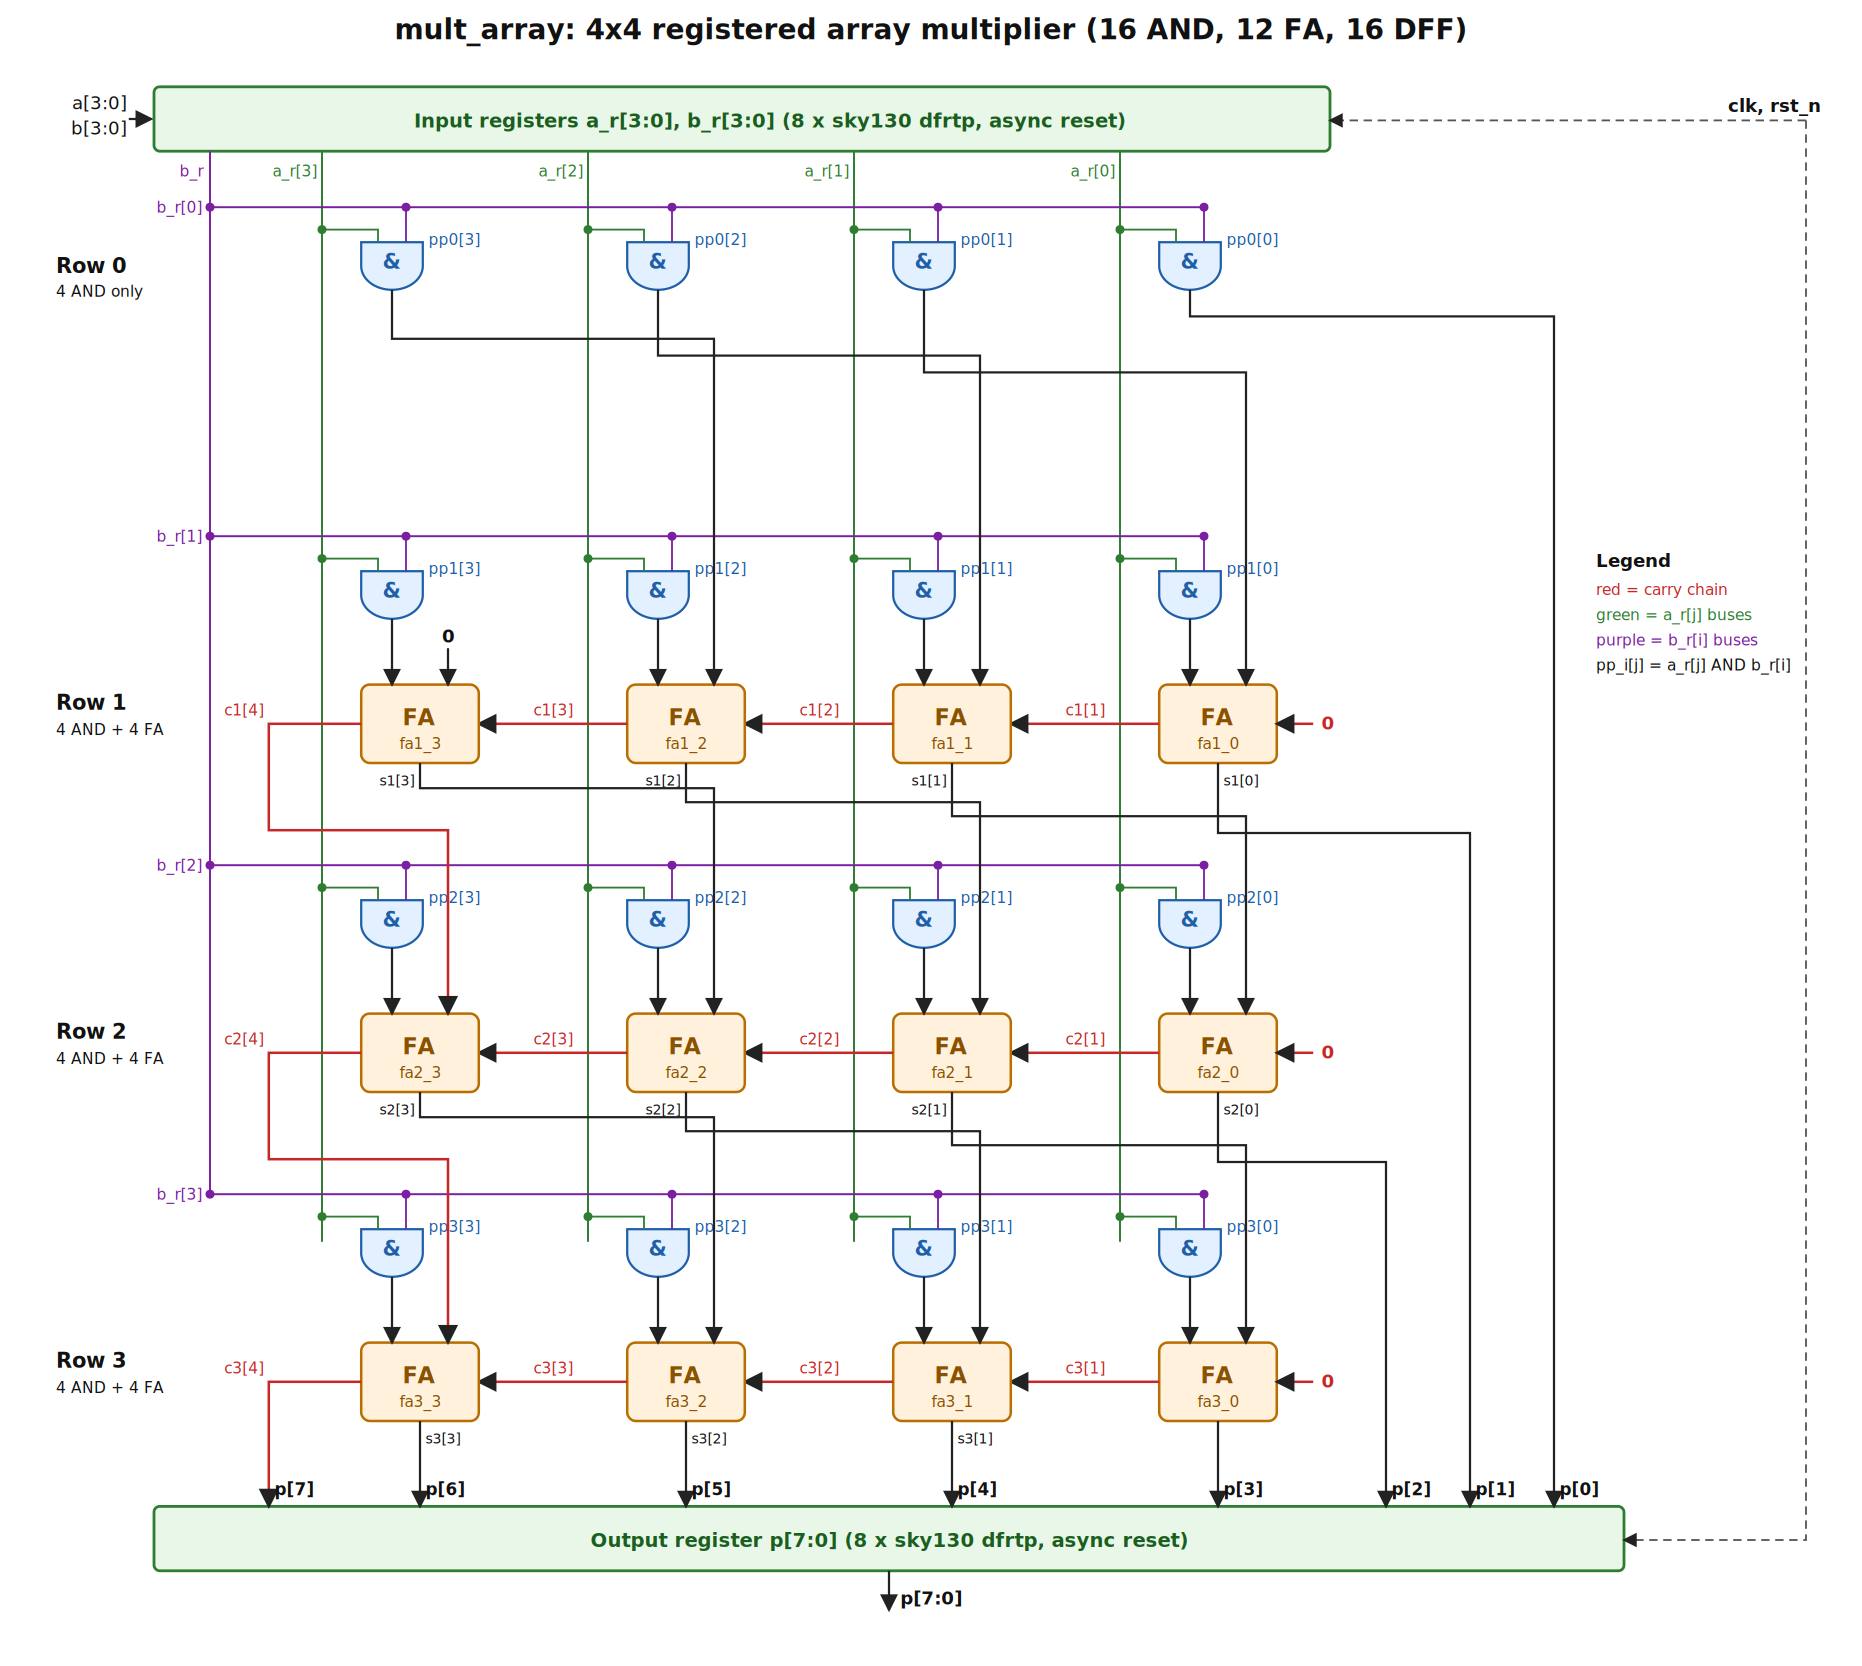
\includegraphics[width=0.82\textwidth]{figures/partA_block_diagram.png}
    \caption{Block diagram of \texttt{mult\_array}: input registers (8 flip-flops), 16 AND gates (blue),
    12 full adders in three ripple-carry rows (orange, carry chains in red) and the output register
    (8 flip-flops).}
    \label{fig:block}
\end{figure*}

\section{Design Flow and Tools}
Table~\ref{tab:tools} lists the tools used. The SKY130 PDK~\cite{sky130} is used with the high-density
standard-cell library \cell{sky130_fd_sc_hd}; synthesis and STA use its typical-corner Liberty file
\cell{sky130_fd_sc_hd__tt_025C_1v80.lib}.

\begin{table}[H]
\centering
\caption{Tools and versions}
\label{tab:tools}
\begin{tabular}{lll}
\toprule
\textbf{Tool} & \textbf{Version} & \textbf{Stage} \\
\midrule
Icarus Verilog~\cite{iverilog} & 14.0 (devel) & RTL / gate-level sim. \\
GTKWave & 3.3.116 & Waveforms \\
Yosys~\cite{yosys} & 0.69 & Synthesis \\
OpenSTA~\cite{opensta} & 3.1.0 & Timing analysis \\
LibreLane~\cite{librelane} & 3.1.0.dev3 & RTL-to-GDSII flow \\
OpenROAD~\cite{openroad} & (in LibreLane) & Place and route \\
Magic~/~Netgen~\cite{magic} & 8.3~/~1.5 & DRC, extraction, LVS \\
KLayout~\cite{klayout} & 0.30 & DRC, layout views \\
\bottomrule
\end{tabular}
\end{table}

\section{RTL Design and Verification}

\subsection{RTL}
\texttt{rtl/full\_adder.v} implements the full adder with two \texttt{assign} statements. \texttt{rtl/mult\_array.v}
(ports \texttt{clk}, \texttt{rst\_n}, \texttt{a[3:0]}, \texttt{b[3:0]}, \texttt{p[7:0]}) contains the input
registers, the 16 AND gates, the 12 explicitly instantiated \texttt{full\_adder}s wired exactly as in
Section~II-B, and the output register (Fig.~\ref{fig:block}). The \texttt{*} operator is not used.

\subsection{Testbench}
The self-checking testbench \texttt{tb/tb\_mult.v}:
\begin{itemize}
    \item generates a 10\,ns clock and holds \texttt{rst\_n} low for the first 2 cycles,
    \item applies all 256 combinations of \texttt{a} and \texttt{b} on the falling edge,
    \item waits two rising edges (the latency) and compares \texttt{p} with \texttt{a*b} 4\,ns after the
          second edge (\texttt{*} is used only in the testbench),
    \item prints every mismatch and one summary line, and writes \texttt{mult.vcd}.
\end{itemize}
The RTL simulation result is:
\begin{footnotesize}
\begin{verbatim}
PASS: 256 vectors checked, 0 errors
\end{verbatim}
\end{footnotesize}

\subsection{Error-Injection Test}
To confirm that the testbench detects errors, \texttt{sum} in \texttt{full\_adder.v} was temporarily changed
to \texttt{a \^{} b}:
\begin{footnotesize}
\begin{verbatim}
MISMATCH at t=1069 ns: a=3 b=3 p=5 expected=9
...
FAIL: 256 vectors checked, 95 errors
\end{verbatim}
\end{footnotesize}
The change was then undone. Only 95 of the 256 products fail, because the bug shows only when a carry-in
of 1 actually reaches a full adder: products such as $x\times0$, $x\times1$ or $x\times2$ never create an
internal carry. Only an exhaustive testbench is guaranteed to expose such a fault. Fig.~\ref{fig:termA}
shows both runs in the terminal.

\begin{figure*}[t]
    \centering
    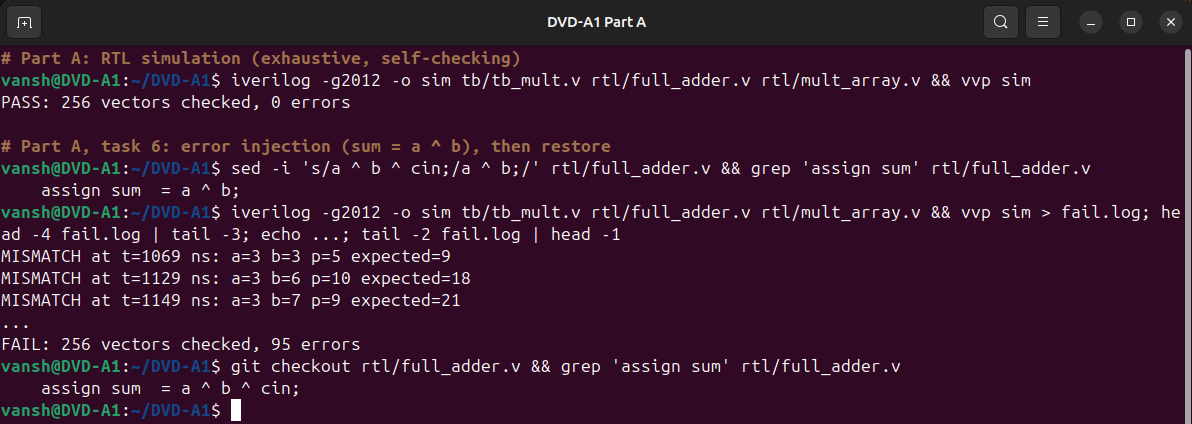
\includegraphics[width=0.85\textwidth]{figures/partA_terminal.png}
    \caption{Terminal output for Part~A: the RTL simulation prints \texttt{PASS: 256 vectors checked, 0 errors};
    with \texttt{sum} changed to \texttt{a \^{} b} the same testbench prints \texttt{FAIL: 256 vectors checked,
    95 errors}, after which the file is restored.}
    \label{fig:termA}
\end{figure*}

\subsection{Hand-Worked Example}
The example uses Vansh Jaiswal's roll number 2024102013 (last digit 3): $A = 3+5 = 8$, $B = 7$.
\begin{footnotesize}
\begin{verbatim}
           1 0 0 0      A = 8
         x 0 1 1 1      B = 7
   ---------------
           1 0 0 0      pp0 (b0 = 1)
         1 0 0 0        pp1 (b1 = 1), << 1
       1 0 0 0          pp2 (b2 = 1), << 2
     0 0 0 0            pp3 (b3 = 0), << 3
   ---------------
   0 0 1 1 1 0 0 0      P = 56
\end{verbatim}
\end{footnotesize}
Table~\ref{tab:trace} traces the same product through the array. Every row matches the simulated internal
signals bit for bit.

\begin{table}[H]
\centering
\caption{$8\times7$ traced through the array}
\label{tab:trace}
\setlength{\tabcolsep}{4pt}
\begin{tabular}{clccc}
\toprule
\textbf{Row} & \textbf{Adds} & \textbf{$s$ / $c[4]$} & \textbf{Bit} & \textbf{Passed down} \\
\midrule
0 & $pp_0 = 1000$ & -- & $p_0=0$ & $r_0 = 0100$ \\
1 & $1000 + 0100$ & $1100$ / 0 & $p_1=0$ & $r_1 = 0110$ \\
2 & $1000 + 0110$ & $1110$ / 0 & $p_2=0$ & $r_2 = 0111$ \\
3 & $0000 + 0111$ & $0111$ / 0 & $p_3=1$ & $p_{7:4} = 0011$ \\
\bottomrule
\end{tabular}
\end{table}
\noindent $P = 0011\,1000_2 = 56 = 8\times7$.

\subsection{Waveform}
Fig.~\ref{fig:wave} shows the example in GTKWave: \texttt{a = 8}, \texttt{b = 7} are applied at 2730\,ns,
captured into \texttt{a\_r}, \texttt{b\_r} at edge~1 (2735\,ns), and \texttt{p = 56} appears at edge~2
(2745\,ns), a latency of 2 clock cycles (20\,ns).

\begin{figure*}[t]
    \centering
    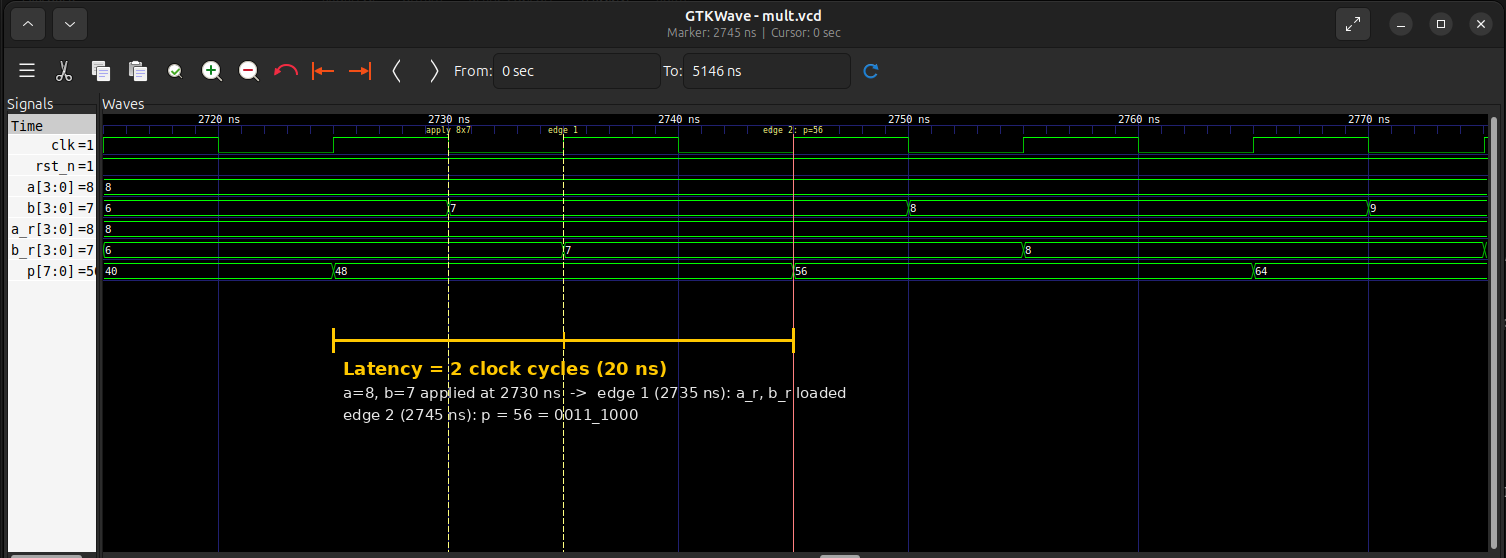
\includegraphics[width=0.95\textwidth]{figures/partA_waveform.png}
    \caption{GTKWave view of the example $8\times7$ with the 2-cycle latency marked: inputs applied at
    2730\,ns, input registers loaded at edge~1 (2735\,ns), \texttt{p = 56} at edge~2 (2745\,ns).}
    \label{fig:wave}
\end{figure*}

\section{Logic Synthesis with Yosys}
\texttt{synth/synth.tcl} runs the seven required Yosys steps: \texttt{read\_verilog},
\texttt{synth -top mult\_array -flatten}, \texttt{dfflibmap} and \texttt{abc} with the Liberty file,
\texttt{opt\_clean -purge}, \texttt{stat -liberty} (saved to \texttt{mult\_array\_stat.rpt}) and
\texttt{write\_verilog -noattr}. The results are in Table~\ref{tab:synth}.

\begin{table}[H]
\centering
\caption{Part B: synthesis results}
\label{tab:synth}
\begin{tabular}{ll}
\toprule
\textbf{Metric} & \textbf{Value} \\
\midrule
Total number of cells & 63 \\
Number of flip-flops & 16 (\cell{sky130_fd_sc_hd__dfrtp_1}) \\
Total cell area & 740.710\umsq \\
Flip-flop area & $16 \times 25.024 = 400.384$\umsq \\
Flip-flop area (\% of total) & 54.05\,\% \\
Top 3 cell types & \cell{dfrtp_1}$\times$16, \cell{nand2_1}$\times$8, \\
 & \cell{a21oi_1}$\times$6 \\
Netlist simulation & \texttt{PASS: 256 vectors, 0 errors} \\
\bottomrule
\end{tabular}
\end{table}

The other 33 cells are \cell{xnor2_1}$\times$4, \cell{maj3_1}$\times$3, \cell{nand3_1}$\times$3,
\cell{xor2_1}$\times$3, \cell{and2_0}$\times$2, \cell{clkinv_1}$\times$2,
\cell{lpflow_isobufsrc_1}$\times$2, \cell{xnor3_1}$\times$2 and 12 cell types used once.

\subsection{Gate-Level Simulation}
The netlist was simulated with the SKY130 cell models (\texttt{-DFUNCTIONAL -DUNIT\_DELAY=\#1}) and the same
testbench, and passes all 256 vectors. The first gate-level run reported every product one vector late.
The cause was in the testbench, not the design: with \texttt{UNIT\_DELAY} the flip-flop models change
\texttt{Q} 1\,ns after the clock edge, exactly when the testbench originally sampled \texttt{p}. Sampling
4\,ns after the edge removed this race; the RTL still passes and the error-injection test still fails.

\section{Static Timing Analysis with OpenSTA}
\texttt{sta/sta.tcl} reads the typical-corner Liberty file and the netlist, defines a clock of period $T$ on
\texttt{clk}, sets 1.0\,ns input and output delays, reports the worst setup slack and saves the
critical-path report. At $T = 10$\,ns the worst slack is 7.396\,ns, so
\begin{align}
T_{min} &= T - WNS = 10 - 7.396 = 2.604~\text{ns}, \\
F_{max} &= 1000 / T_{min} = 384.0~\text{MHz}.
\end{align}
Rerunning at $T = 2.60$\,ns ($T_{min}$ rounded to 0.01\,ns) gives a slack of $-0.004$\,ns $\approx 0$, and
2.61\,ns gives $+0.006$\,ns. With an ideal clock the path delay does not depend on $T$, so the slack is
exactly $T - 2.604$\,ns. Fig.~\ref{fig:termBC} shows the gate-level simulation and both STA runs in the
terminal.

\begin{figure*}[t]
    \centering
    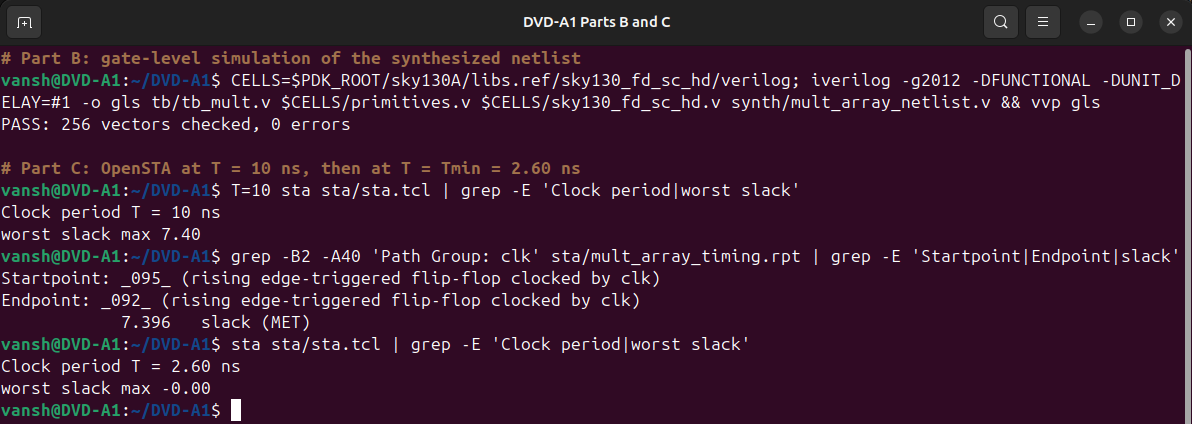
\includegraphics[width=0.85\textwidth]{figures/partBC_terminal.png}
    \caption{Terminal output for Parts~B and~C: the gate-level netlist simulation passes all 256 vectors; OpenSTA
    reports a worst slack of 7.40\,ns (7.396\,ns in the report) at $T = 10$\,ns, from \texttt{\_095\_}
    (\texttt{a\_r[1]}) to \texttt{\_092\_} (\texttt{p[6]}), and $-0.00$\,ns at $T = T_{min} = 2.60$\,ns.}
    \label{fig:termBC}
\end{figure*}

\begin{table}[H]
\centering
\caption{Part C: timing results (tt\_025C\_1v80)}
\label{tab:sta}
\begin{tabular}{ll}
\toprule
\textbf{Metric} & \textbf{Value} \\
\midrule
Worst slack at $T = 10$\,ns & 7.396\,ns \\
$T_{min}$ & 2.604\,ns ($\approx$ 2.60\,ns) \\
$F_{max}$ & 384.0\,MHz \\
Slack at $T = T_{min}$ & $-0.004$\,ns ($\approx 0$) \\
Critical path start point & \texttt{a\_r[1]} register (CLK) \\
Critical path end point & \texttt{p[6]} register (D) \\
Cells on the critical path & 9 (launch flip-flop + 8 gates) \\
Latency $= 2\,T_{min}$ & 5.208\,ns \\
Throughput & 384.0 million results/s \\
\bottomrule
\end{tabular}
\end{table}

\subsection{Critical Path}
Table~\ref{tab:path} lists the cells on the critical path. Each net was matched to an RTL signal by comparing
its truth table over all 256 values of (\texttt{a\_r}, \texttt{b\_r}) with the equations of Section~II.

\begin{table}[H]
\centering
\caption{Critical path cells ($T = 10$\,ns report)}
\label{tab:path}
\setlength{\tabcolsep}{3.5pt}
\begin{tabular}{clrrll}
\toprule
\textbf{\#} & \textbf{Cell} & \textbf{Delay} & \textbf{Arr.} & \textbf{Signal} & \textbf{Part of} \\
 & & \textbf{(ns)} & \textbf{(ns)} & & \\
\midrule
0 & \cell{dfrtp_1} & 0.398 & 0.398 & \texttt{a\_r[1]} & input reg. \\
1 & \cell{clkinv_1} & 0.074 & 0.472 & $\overline{a\_r[1]}$ & AND gates \\
2 & \cell{o311ai_0} & 0.348 & 0.820 & merged & AND + fa1\_1 \\
3 & \cell{a21oi_1} & 0.172 & 0.992 & $c_2[1]$ & fa2\_0 carry \\
4 & \cell{maj3_1} & 0.381 & 1.373 & $c_2[2]$ & fa2\_1 carry \\
5 & \cell{xnor2_1} & 0.160 & 1.534 & $\overline{s_2[2]}$ & fa2\_2 sum \\
6 & \cell{maj3_1} & 0.385 & 1.918 & $\overline{c_3[2]}$ & fa3\_1 carry \\
7 & \cell{maj3_1} & 0.377 & 2.295 & $\overline{c_3[3]}$ & fa3\_2 carry \\
8 & \cell{xnor3_1} & 0.175 & 2.471 & $s_3[3]$ & fa3\_3 sum \\
\bottomrule
\end{tabular}
\end{table}

The path delay is $0.398$ (clock-to-Q) $+\ 2.073$ (logic) $+\ 0.134$ (setup) $= 2.605$\,ns $\approx T_{min}$.
It crosses \textbf{7 full-adder stages}, fa1\_1 $\rightarrow$ fa2\_0 $\rightarrow$ fa2\_1 $\rightarrow$
fa2\_2 $\rightarrow$ fa3\_1 $\rightarrow$ fa3\_2 $\rightarrow$ fa3\_3: along the row-2 carry chain, down
through $s_2[2]$, and along the row-3 carry chain to the top sum bit. This agrees well with the estimate of
about $2N = 8$ full-adder delays. Six of the eight gates compute a full-adder carry or sum directly, and each
stage costs only one gate ($\approx 0.30$\,ns) because the path needs either the carry or the sum of each
adder, not both.

\section{Physical Design with LibreLane}

\subsection{Configuration and Runs}
\texttt{pnr/config.json} sets:
\begin{itemize}
    \item \texttt{DESIGN\_NAME}: \texttt{mult\_array}; \texttt{CLOCK\_PORT}: \texttt{clk},
    \item \texttt{VERILOG\_FILES}: the two RTL files,
    \item \texttt{FP\_SIZING}: \texttt{absolute}; \texttt{DIE\_AREA}: $[0,0,150,150]$, a fixed $150\times150$\um\ die,
    \item \texttt{CLOCK\_PERIOD}: started at $1.2\,T_{min} = 3.125$\,ns, rounded up to 3.5\,ns.
\end{itemize}
The flow was run with \texttt{librelane config.json}, and the clock period was increased by 0.5\,ns after
every failing run (Table~\ref{tab:runs}).

\begin{table}[H]
\centering
\caption{LibreLane runs (slack in ns)}
\label{tab:runs}
\setlength{\tabcolsep}{4.5pt}
\begin{tabular}{ccrrccl}
\toprule
\textbf{Run} & \textbf{Period} & \textbf{Worst} & \textbf{Typ.} & \textbf{DRC} & \textbf{LVS} & \textbf{Result} \\
 & \textbf{(ns)} & \textbf{slack} & \textbf{slack} & & & \\
\midrule
1 & 3.5 & $-2.132$ & $+0.547$ & 0 & 0 & fail \\
2 & 4.0 & $-1.632$ & $+1.047$ & 0 & 0 & fail \\
3 & 4.5 & $-1.142$ & $+1.551$ & 0 & 0 & fail \\
4 & 5.0 & $-0.642$ & $+2.052$ & 0 & 0 & fail \\
5 & 5.5 & $-0.142$ & $+2.552$ & 0 & 0 & fail \\
6 & 6.0 & $-0.064$ & $+2.943$ & 0 & 0 & fail \\
\textbf{7} & \textbf{6.5} & $\mathbf{+0.085}$ & $\mathbf{+3.293}$ & \textbf{0} & \textbf{0} & \textbf{pass} \\
\bottomrule
\end{tabular}
\end{table}

DRC and LVS were clean in every run; only setup timing failed, and only in the slow corner
\cell{max_ss_100C_1v60} (slow transistors, 100\,\textdegree C, 1.60\,V). LibreLane signs off in 9 corners and
reports the worst as \texttt{setup\_\_ws}; the typical corner of Part~C passed from the first run. Runs 1--5
gained almost exactly 0.5\,ns per step, but run 6 gained only 0.08\,ns: LibreLane re-synthesises and re-sizes
the design for each target period and uses smaller, slower gates when the clock is loose.

\subsection{Results}
\begin{table}[H]
\centering
\caption{Part D: physical-design results}
\label{tab:pnr}
\begin{tabular}{ll}
\toprule
\textbf{Metric} & \textbf{Value} \\
\midrule
CLOCK\_PERIOD used & 6.5\,ns \\
Number of runs needed & 7 \\
Core area & 17\,759.5\umsq\ (die 22\,500\umsq) \\
Cells after synthesis (Part B) & 63 \\
Cells after place and route & 1\,901 \\
Kinds of cells added & decap, fill, tap, I/O, clock \\
 & and fanout buffers (Table~\ref{tab:cells}) \\
Wirelength & 2\,405\um \\
Setup slack (worst corner) & $+0.085$\,ns \\
Post-route $F_{max}$ & $1000/(6.5-0.085) = 155.9$\,MHz \\
$F_{max}$ from Part C & 384.0\,MHz \\
DRC errors & 0 (Magic, KLayout, router) \\
LVS errors & 0 (Netgen) \\
\bottomrule
\end{tabular}
\end{table}

Further signoff results: hold slack $+0.124$\,ns, no antenna or power-grid violations, identical Magic and
KLayout GDS streams (XOR difference 0), and 7.0\,\% cell utilisation. The flow also reported 11 max-slew
warnings, all in the slow corner and all on the asynchronous reset net (0.761\,ns transition against a
0.75\,ns limit); the typical corner has none and the flow completed successfully.

\begin{table}[H]
\centering
\caption{Cells after place and route}
\label{tab:cells}
\setlength{\tabcolsep}{4pt}
\begin{tabular}{llr}
\toprule
\textbf{Kind} & \textbf{Cells} & \textbf{Count} \\
\midrule
Tap & \cell{tapvpwrvgnd_1} & 245 \\
Decap & \cell{decap_3/4/6/8/12} & 1\,296 \\
Fill & \cell{fill_1}, \cell{fill_2} & 270 \\
Clock-tree buffers & \cell{clkbuf_16} & 3 \\
I/O buffers & \cell{buf_2} (9 in, 8 out) & 17 \\
Fanout buffers & \cell{clkdlybuf4s50_1} & 2 \\
Design cells & \cell{dfrtp_1}, logic, \cell{inv_1} & 68 \\
\midrule
\textbf{Total} & & \textbf{1\,901} \\
\bottomrule
\end{tabular}
\end{table}

LibreLane runs its own synthesis script, which produced 68 design cells (16 flip-flops, 49 logic gates,
3 inverters) instead of the 63 of Part~B.

\subsection{Layout}
Fig.~\ref{fig:die} shows the whole die and Fig.~\ref{fig:zoom} a zoomed view of the logic.

\begin{figure}[H]
    \centering
    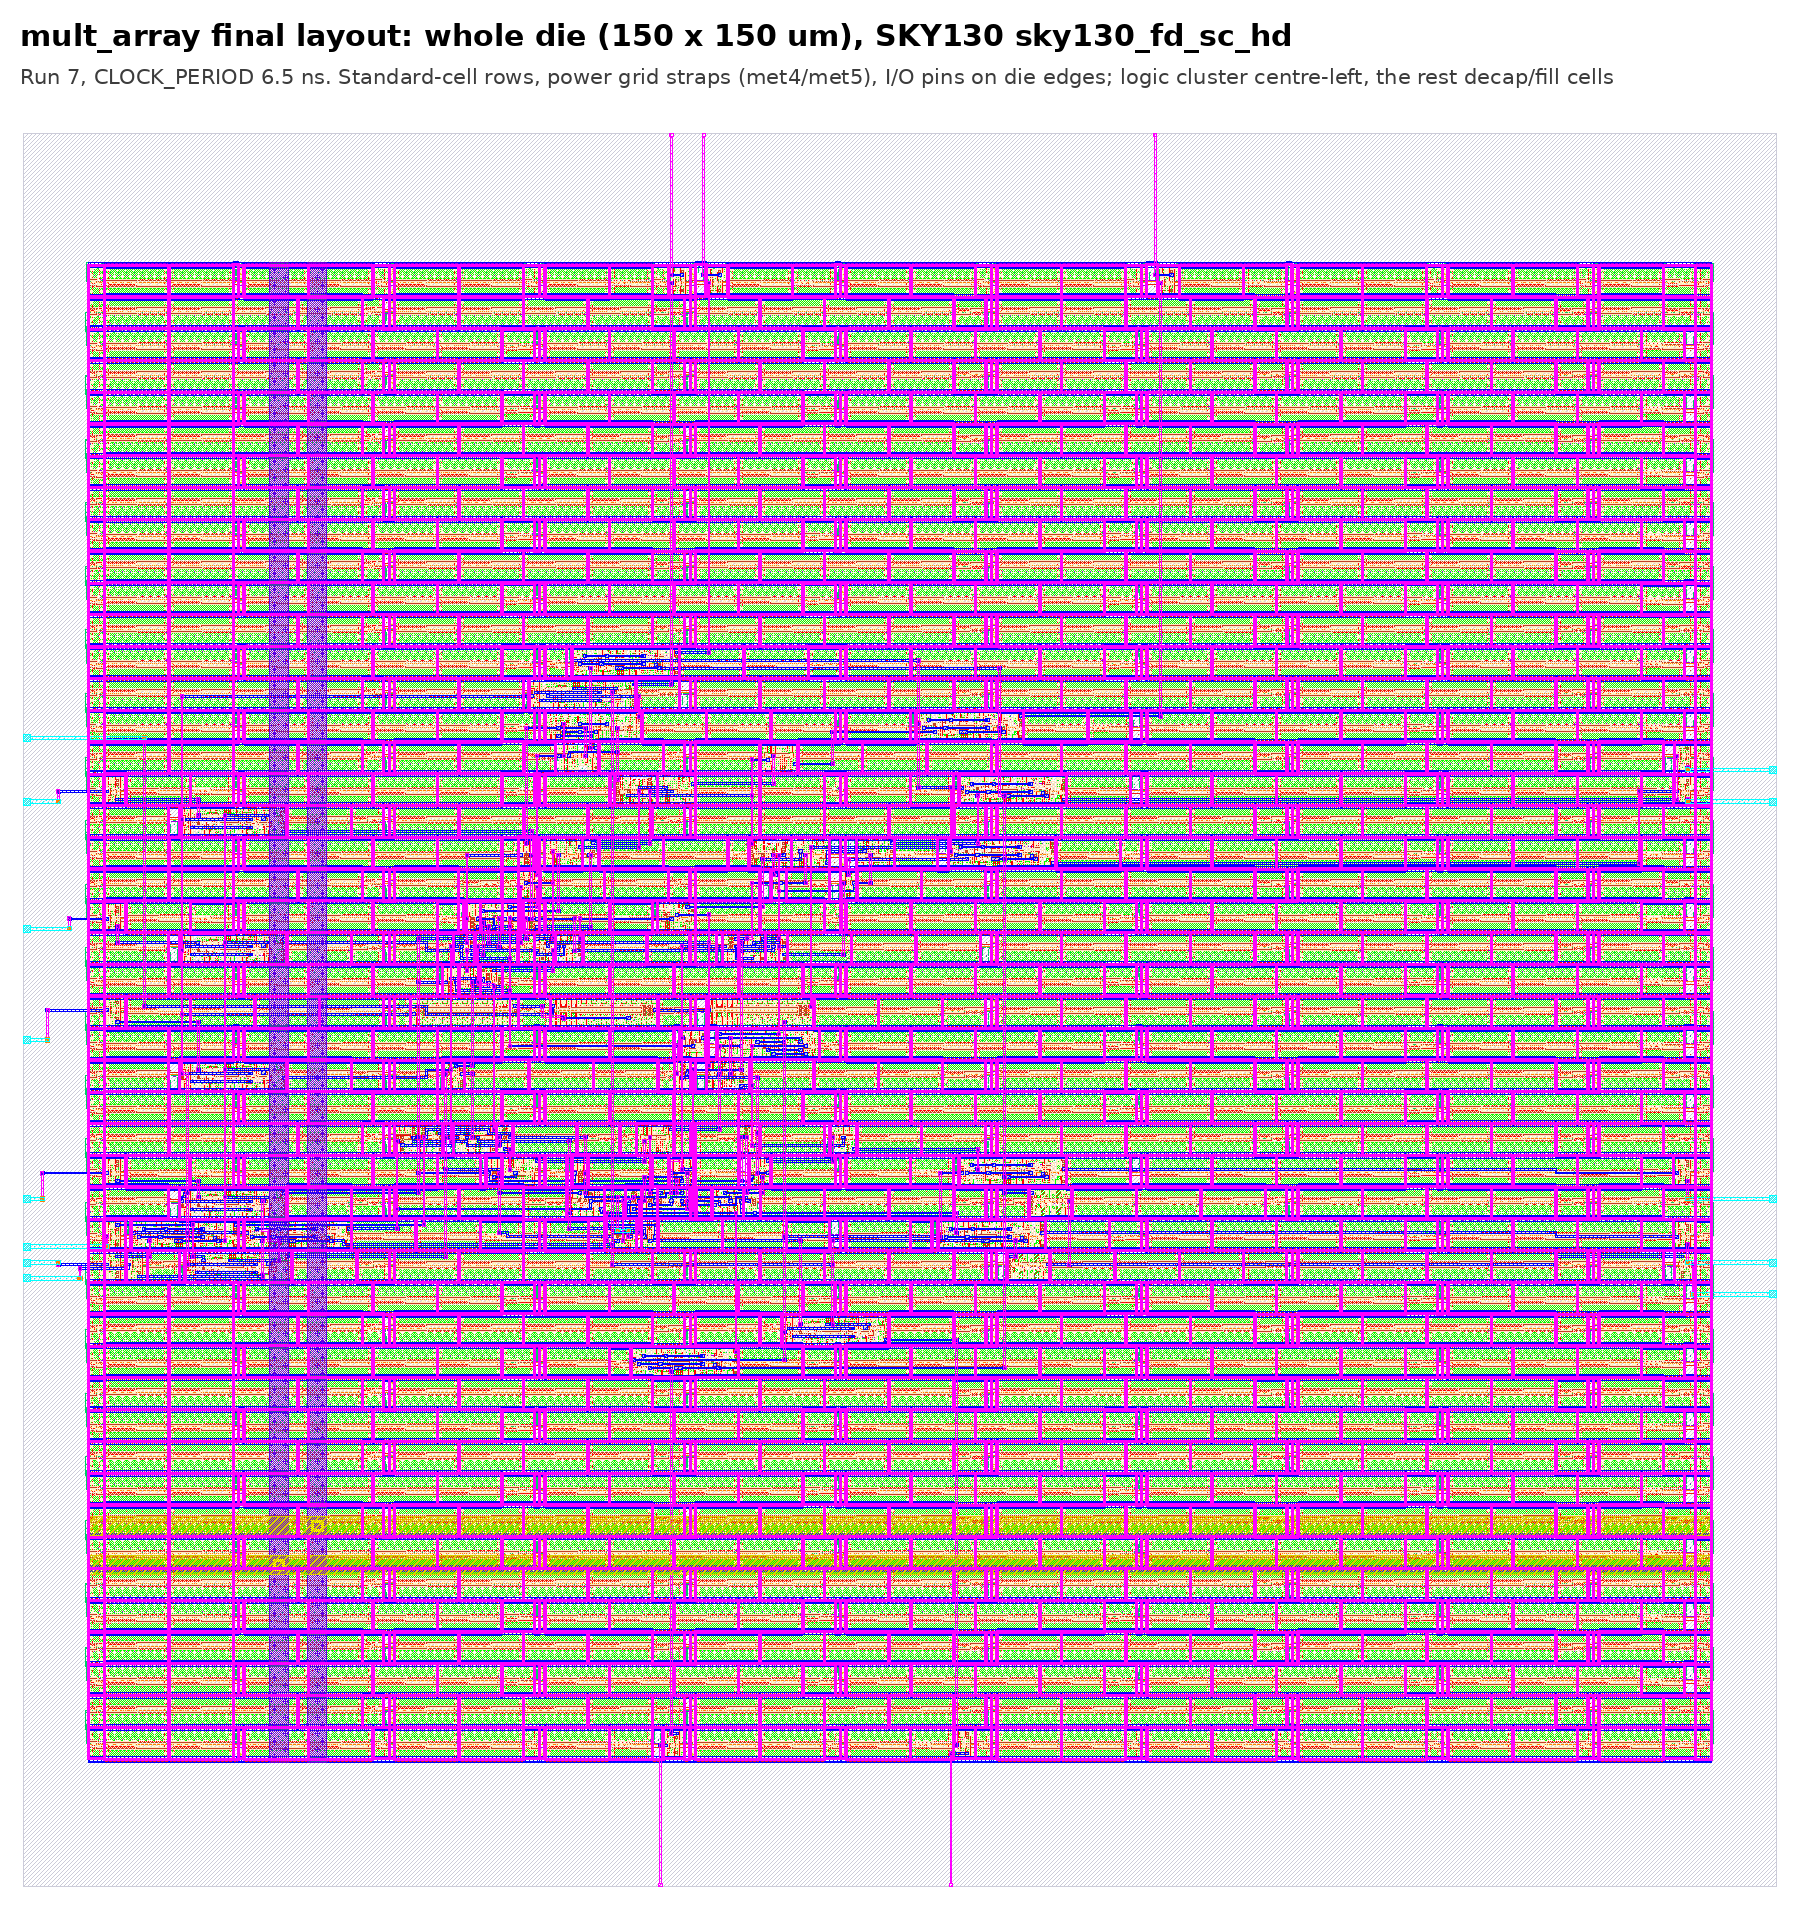
\includegraphics[width=0.48\textwidth]{figures/partD_layout_die.png}
    \caption{Final layout, whole $150\times150$\um\ die (KLayout). Standard-cell rows under the power-grid
    straps and I/O pins on the die edges; the logic sits centre-left and the remaining space is decap and
    fill cells.}
    \label{fig:die}
\end{figure}

\begin{figure}[H]
    \centering
    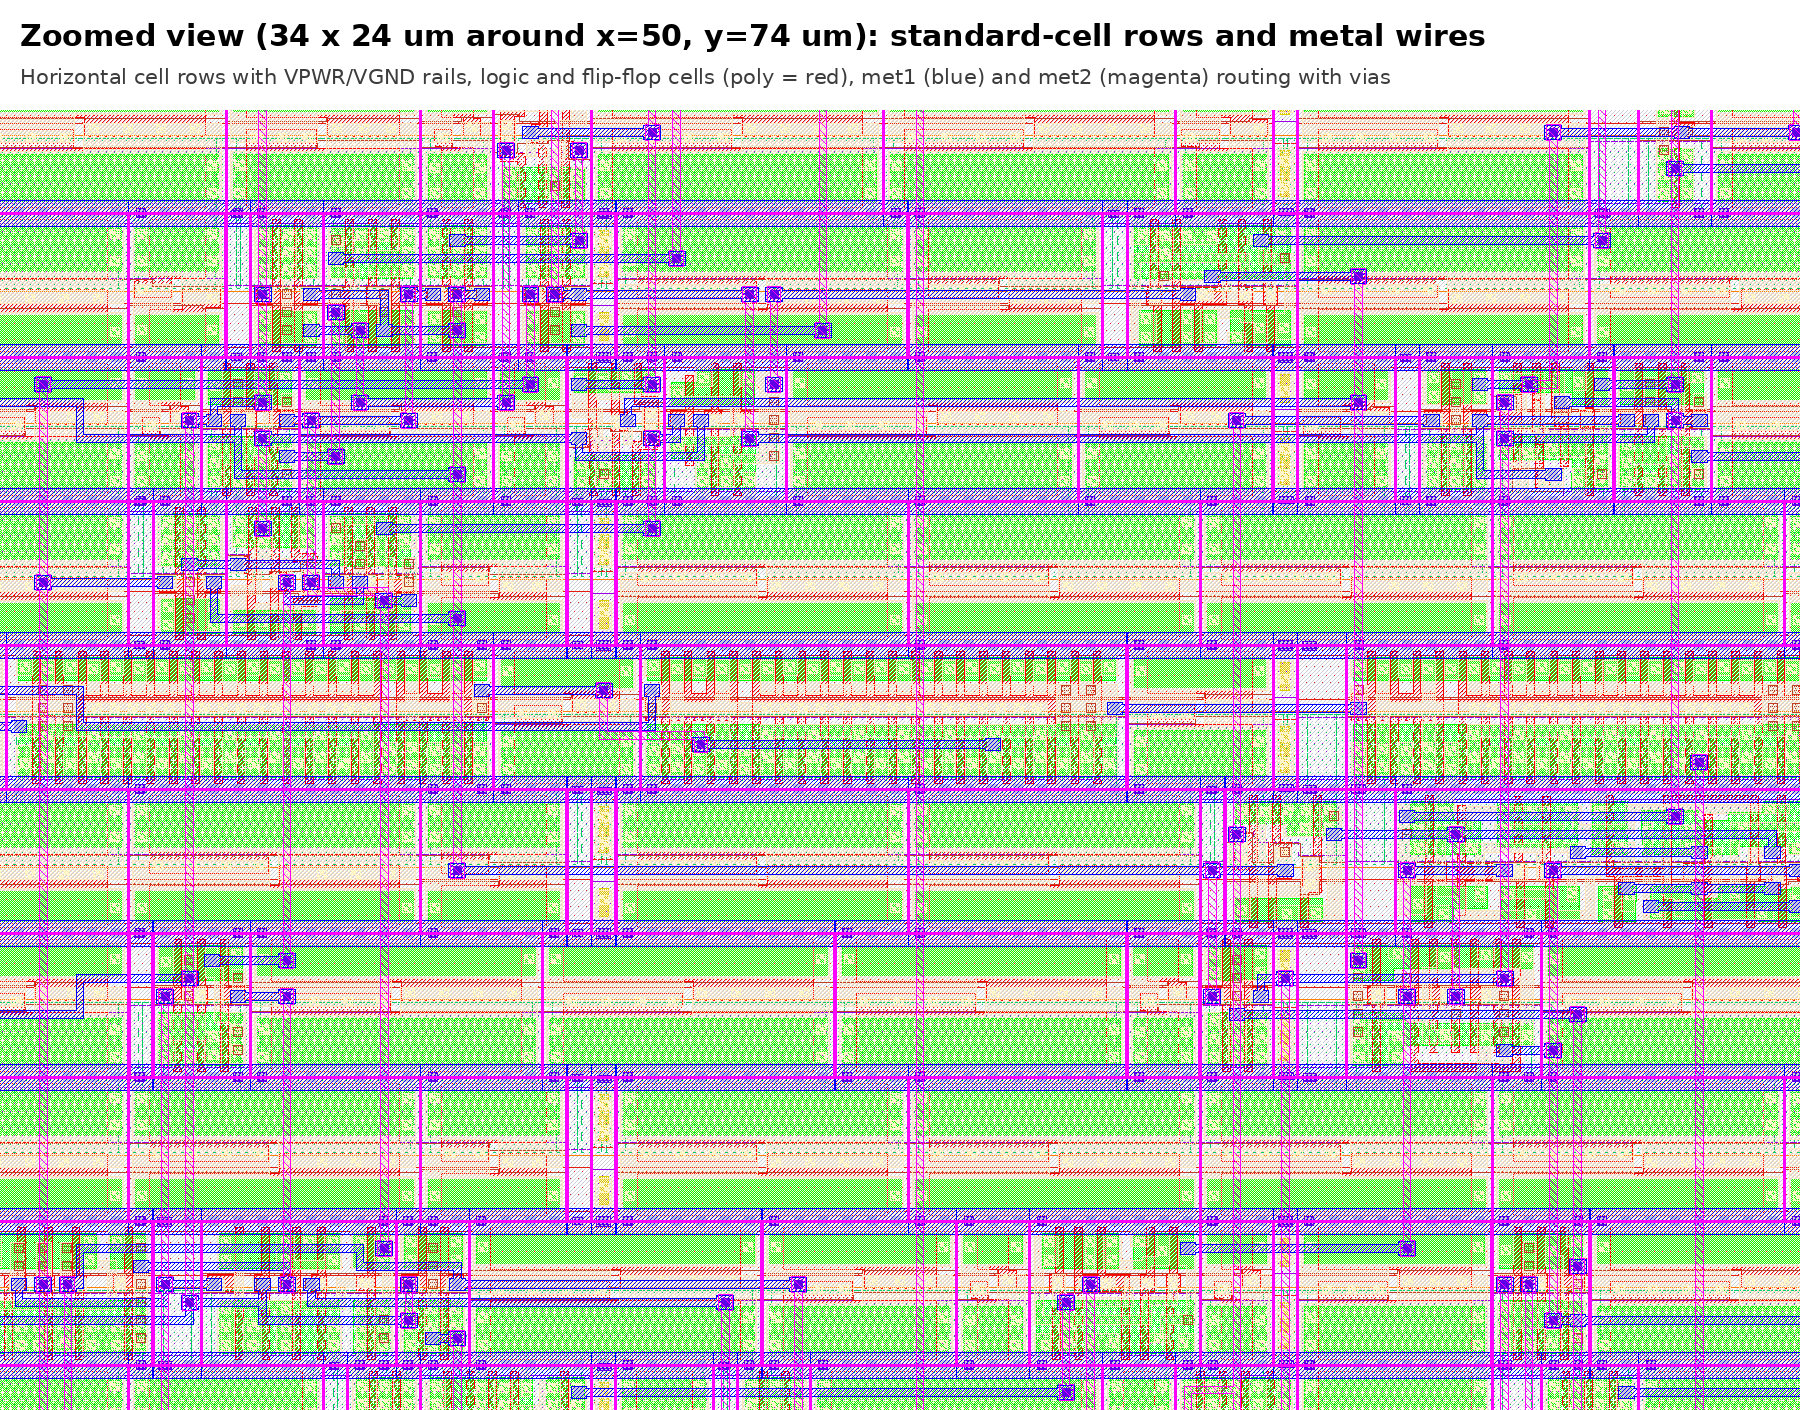
\includegraphics[width=0.48\textwidth]{figures/partD_layout_zoom.png}
    \caption{Zoomed view ($34\times24$\um\ around the logic): standard-cell rows with VPWR/VGND rails,
    logic and flip-flop cells (polysilicon in red), metal-1 (blue) and metal-2 (magenta) wires with vias.}
    \label{fig:zoom}
\end{figure}

\section{Answers to the Questions}

\subsection{Q1: Logic Cells after Synthesis}
Synthesis produced $63 - 16 = $ \textbf{47 logic cells} (340.3\umsq) for 16 AND gates and 12 full adders
(28 blocks). The numbers differ because ABC maps the flattened logic onto library cells rather than onto
our modules. ABC does not use the multi-output full-adder cell (\cell{fa_1}), so each adder becomes a sum
gate (\cell{xor}/\cell{xnor}, sometimes \cell{xor3}/\cell{xnor3}) plus a carry gate (\cell{maj3} or
AOI/OAI/NAND logic), which raises the count. In the other direction, many AND gates are absorbed into
complex gates (\cell{o311ai}, \cell{a21oi}, \cell{nand2}), the column-0 adders have $c_{in} = 0$ and reduce
to half adders, and the constant 0 fed into row 1 removes logic, which lowers it. Two inverters
(\cell{clkinv_1}) fix polarities. The resulting netlist is logically identical to the RTL, as the
256-vector gate-level simulation confirms.

\subsection{Q2: Critical Path}
The critical path runs from the \textbf{\texttt{a\_r[1]} input register} to the \textbf{\texttt{p[6]} output
register} and contains \textbf{9 cells}: the launch flip-flop and 8 gates (\cell{clkinv}, \cell{o311ai},
\cell{a21oi}, \cell{maj3}, \cell{xnor2}, \cell{maj3}, \cell{maj3}, \cell{xnor3}), with an arrival time of
2.471\,ns and a 0.134\,ns setup time at the typical corner. Matching every net to the RTL shows that it
crosses \textbf{7 full-adder stages}, along the row-2 carry chain, through $s_2[2]$ into row 3 and along the
row-3 carry chain to $s_3[3]$. This is close to the estimate of about $2N = 8$ full-adder delays, which is
only an approximation of the longest chain. Each stage costs a single gate ($\approx 0.30$\,ns) because the
path uses only the carry or only the sum of each adder.

\subsection{Q3: Flip-Flop Area}
The flip-flops occupy $400.384/740.710 = $ \textbf{54.05\,\%} of the cell area, although they are only 16 of
the 63 cells. A \cell{dfrtp_1} is a master--slave flip-flop with asynchronous reset; at 25.02\umsq\ it is the
largest cell in the design, about 6.7 times a \cell{nand2_1} (3.75\umsq) and larger than any combinational
cell used (the largest is \cell{xor3_1} at 23.77\umsq). The design is also very small: the array has only
28 AND/full-adder blocks, while registering both inputs and the output needs $4N = 16$ flip-flops. Registers
grow linearly with $N$ but the array grows as $N^2$; for $N = 8$ we would expect 32 flip-flops
(800.8\umsq) against about 120 blocks ($\approx 1460$\umsq\ at our 12.15\umsq\ per block), so the
flip-flop share would fall to about 35\,\%.

\subsection{Q4: Post-Route versus Pre-Layout $F_{max}$}
The post-route $F_{max}$ is \textbf{155.9\,MHz} against \textbf{384.0\,MHz} in Part~C, because Part~C was an
idealised analysis:
\begin{enumerate}
    \item \emph{Corner:} Part~C used only the typical corner, while LibreLane signs off in the slow corner
          (100\,\textdegree C, 1.60\,V), where the cells are about twice as slow. In the typical corner alone the
          routed design reaches $1000/(6.5-3.293) = 311.8$\,MHz.
    \item \emph{Wires:} routed nets add resistance and capacitance, increasing gate delay and slew.
    \item \emph{Clock:} instead of an ideal clock, the clock passes through two levels of \cell{clkbuf_16}
          ($\approx 0.5$\,ns latency, with skew between flip-flops), and the flow adds 0.25\,ns of clock
          uncertainty.
    \item \emph{Netlist:} LibreLane re-synthesises for the target period and uses smaller, slower gates when
          the clock is loose.
\end{enumerate}
The flow added 1\,833 cells (68 $\rightarrow$ 1\,901). \emph{Tap cells} (245) tie the n-well to VPWR and the
substrate to VGND at regular intervals in every row to prevent latch-up. \emph{Decap cells} (1\,296) are
capacitors between VPWR and VGND that supply charge locally when gates switch, reducing supply noise and
IR drop. \emph{Fill cells} (270) close the remaining gaps so that wells, implants and power rails are
continuous along each row, as required by DRC. \emph{Buffers}: three \cell{clkbuf_16} form the clock tree
that delivers \texttt{clk} to all 16 flip-flops with low skew, 17 \cell{buf_2} I/O buffers isolate the 9
input and 8 output pins from the internal logic, and two fanout buffers split the high-fanout reset net.

\subsection{Q5: DRC and LVS}
\emph{Design rule checking} (DRC) verifies that the layout geometry obeys the foundry's manufacturing rules:
minimum widths and spacings of every layer, enclosures of contacts and vias, overlaps and densities.
\emph{Layout versus schematic} (LVS) extracts the transistors and their connections from the layout and
checks that they form exactly the same circuit as the gate-level netlist, with the same devices, nets and
pins. A DRC violation means the chip may not be manufacturable or will suffer shorts and opens that lower
yield; an LVS mismatch means that a perfectly manufacturable chip would implement the wrong circuit. A
layout can pass one check and fail the other, so both must pass before tape-out. Our final layout has
\textbf{0 DRC errors} (Magic, KLayout and the router) and \textbf{0 LVS errors} (Netgen).

\subsection{Q6: Scaling to 8 Bits}
With $N = 8$ instead of $N = 4$:
\begin{align}
\text{Full adders: } & N(N-1) = 8\times7 = \mathbf{56} \quad (\text{vs. } 4\times3 = 12), \\
\text{AND gates: } & N^2 = 64 \quad (\text{vs. } 16), \\
\text{Critical path: } & \approx 2N = \mathbf{16}\ \text{FA delays} \quad (\text{vs. } 8).
\end{align}
The number of full adders grows 4.7 times (quadratically), while the critical path only doubles
(linearly), and the flip-flop count doubles to $4N = 32$. With our measured values (0.398\,ns clock-to-Q,
$\approx 0.296$\,ns per full-adder stage, 0.134\,ns setup):
\begin{equation}
T_{min,8} \approx 0.398 + 16\times0.296 + 0.134 = 5.27~\text{ns},
\end{equation}
i.e.\ $F_{max} \approx 190$\,MHz at the typical corner, compared with 2.604\,ns and 384.0\,MHz for the 4-bit
design.

\section{Conclusion}
A registered 4-bit array multiplier was taken through a complete open-source RTL-to-GDSII flow in SKY130:
\begin{enumerate}
    \item RTL design with 16 AND gates and 12 full adders, verified exhaustively (256/256) with a testbench
          that provably detects injected faults,
    \item synthesis to 63 standard cells (740.71\umsq) with a passing gate-level simulation,
    \item static timing analysis giving $T_{min} = 2.604$\,ns ($F_{max} = 384.0$\,MHz) with a critical path
          through 7 full-adder stages, close to the $2N$ estimate,
    \item place and route to a DRC- and LVS-clean $150\times150$\um\ layout that meets multi-corner setup
          timing at 6.5\,ns (155.9\,MHz).
\end{enumerate}
The drop from 384.0\,MHz to 155.9\,MHz shows how strongly signoff conditions that the pre-layout analysis
ignores (the slow process corner, interconnect parasitics, the real clock tree and clock uncertainty) limit
the achievable clock frequency, and why post-layout analysis is essential in practical VLSI design.

\section{Individual Contributions}
The work was divided equally between the two team members. By the assignment's own weighting, each member
owns 50 of the 100 marks: Parts~A and~C ($30+20$) and Parts~B and~D ($20+30$). Each member also answered
the questions that belong to their own parts:
\begin{itemize}\raggedright
    \item \textbf{Vansh Jaiswal (2024102013):} Part~A (\texttt{full\_adder.v}, \texttt{mult\_array.v}, the
          self-checking testbench and its sampling fix, the error-injection test, the hand-worked example and
          the waveform figure) and Part~C (\texttt{sta.tcl}, $T_{min}$ and $F_{max}$, tracing the critical path
          through the full-adder stages); answers to Q2 and Q6; the GitHub repository and the README command log.
    \item \textbf{Saarthak Sabharwal (2023102055):} Part~B (\texttt{synth.tcl}, synthesis, gate-level
          simulation and the cell/area table) and Part~D (\texttt{config.json}, the LibreLane runs, the
          added-cell analysis, layout inspection in Magic and KLayout, DRC/LVS signoff and the layout figures);
          the block diagram; answers to Q1, Q3, Q4 and Q5; review of the pull request.
\end{itemize}
Both members wrote the report and cross-checked each other's results. All commits were pushed from Vansh's
GitHub account, so the commit history shows a single author.

\section*{Acknowledgment}
We thank the course instructor and the teaching assistants of Digital VLSI Design for their guidance, and
the developers of the open-source EDA tools and the SkyWater PDK used in this work.

\section*{Use of AI Tools}
An AI assistant was used to support parts of this work. The team guided it throughout, reviewed and verified
every step and result, and takes full responsibility for the submitted design and report, in line with the
responsible use of AI.

\begin{thebibliography}{00}
\bibitem{weste}
N.~Weste and D.~Harris, \emph{CMOS VLSI Design: A Circuits and Systems Perspective}, 4th~ed. Pearson,
ch.~11.
\bibitem{rabaey}
J.~Rabaey, A.~Chandrakasan and B.~Nikoli\'c, \emph{Digital Integrated Circuits: A Design Perspective},
2nd~ed. Pearson.
\bibitem{iic}
``IIC-OSIC-TOOLS.'' [Online]. Available: \url{https://github.com/iic-jku/IIC-OSIC-TOOLS}
\bibitem{sky130}
``SkyWater SKY130 PDK.'' [Online]. Available: \url{https://skywater-pdk.readthedocs.io}
\bibitem{iverilog}
``Icarus Verilog.'' [Online]. Available: \url{https://steveicarus.github.io/iverilog}
\bibitem{yosys}
``Yosys Open SYnthesis Suite.'' [Online]. Available: \url{https://yosyshq.readthedocs.io/projects/yosys}
\bibitem{opensta}
``OpenSTA.'' [Online]. Available: \url{https://github.com/parallaxsw/OpenSTA}
\bibitem{librelane}
``LibreLane.'' [Online]. Available: \url{https://github.com/librelane/librelane}
\bibitem{openroad}
``OpenROAD.'' [Online]. Available: \url{https://openroad.readthedocs.io}
\bibitem{magic}
``Magic VLSI Layout Tool and Netgen.'' [Online]. Available: \url{http://opencircuitdesign.com}
\bibitem{klayout}
``KLayout.'' [Online]. Available: \url{https://www.klayout.de}
\end{thebibliography}

\end{document}
